\section{연구 과정}

\subsection{라즈베리파이에 운영체제 설치 및 네트워크 설치}
\subsubsection{라즈비안 설치 및 기본 설정}
인터넷을 통해 라즈베리파이의 OS인 라즈비안 4.19, 라즈베리파이를 외부 컴퓨터에서 원격으로 접속하기 위한 VNC Viewer, 마이크로 SD 카드에 운영 체제를 전달하기 위한 balena Etcher v1.5.56을 내려받았다. balena Etcher를 사용해 라즈비안 파일을 마이크로 SD로 전송하고, SD카드는 라즈베리 파이에 삽입하여 라즈베리파이를 구동하였다. 라즈베리파이 2개에 OS를 설치하였으나 실제 센서 연결 및 프로그래밍은 하나의 라즈베리파이에서만 하였다.
구동 후 라즈베리파이에 HDMI선을 이용하여 모니터와 연결한 후 기본 설정을 하였다. 

라즈베리파이 장비의 이름은 각각 AWS-01과 AWS-02로 하였고, 외부 접속 비밀번호를 설정하였다. Raspberry pi 3의 경우 WiFi 지역 설정을 한국으로 하면 접속이 되지 않는 오류가 있어 부득이하게 지역을 영국으로 하되 시간은 서울의 표준 시각(KST)을 사용하였다. 라즈베리파이에 GSHS\_AWS1 공유기를 연결한 후 라즈베리파이의 내부 IP 주소가 각각 192.168.0.6과 192.168.0.4임을 확인해 노트북의 VNC Viewer를 사용하여 원격 접속하였다. VNC Viewer의 사용을 위해서는 라즈베리 파이 설정에서 VNC를 허용해야 한다.

\subsubsection{네트워크 및 공유기 설정}
라즈베리파이에서 수집한 정보를 서버로 전송하고 개인 노트북으로 라즈베리파이에 접속해 명령어 작업을 하기 위하여 라즈베리파이를 Wi-Fi 공유기 ‘GSHS\_AWS1’에 새로 연결시켰다. 공유기의 IP는 192.168.0.1이다. 그 후 공유기의 DHCP 설정 페이지에서 라즈베리파이의 내부 IP 주소를 AWS-01은 192.168.0.101, AWS-02는 192.168.0.102로 고정시켰다. 라즈베리파이의 네트워크 설정(Network Prefernces)에서도 IPv4 주소를 AWS-02 기준으로 192.168.0.102, 라우터 주소를 192.168.0.1, DNS 주소를 168.126.63.1로 설정하였다. 라즈베리파이에 모니터를 연결하지 않고도 외부 컴퓨터에서 작업을 하기 위해서는 컴퓨터에 VNC Viewer를 설치 후 라즈베리파이에 연결해야 한다. 컴퓨터의 네트워크를 GSHS-AWS01에 연결 후 VNC Viewer에서 라즈베리파이에 접속하기 위해 라즈베리파이의 내부 IP 주소인 192.168.0.102를 입력하였다. 그 후 사용자 이름에 pi를 입력하고 설정한 비밀번호를 입력했을 때 정상적으로 접속이 됨을 확인하였다.

\subsection{센서의 연결}

라즈베리파이에 각종 기상 정보를 수집할 수 있는 센서를 연결한 후 센서에서 수집한 자료를 처리하는 프로그램을 코딩하였다.

% Please add the following required packages to your document preamble:
% \usepackage{graphicx}
\begin{table}[htbp]
	\caption{연구에서 사용한 센서의 목록}
	\label{SENSOR}
	\resizebox{\textwidth}{!}{%
		\begin{tabular}{c|c|c|c|c}
		\toprule
			측정 자료 & 센서 이름     & 동작 전압          & 핀 사용량                    & 비고                    \\ 
		\toprule
			온습도   & dht22     & 3.3 $\textrm{V}$           & 3                        & 10kΩ 저항 사용            \\ \hline
			기압    & BMP180    & 3.3 $\textrm{V}$           & 6 (SPI 사용시), 4 (I2C 사용시) &                       \\ \hline
			미세먼지  & PMS7003   & 5 $\textrm{V}$             & -                        & UART 통신 사용, USB 포트 사용 \\ \hline
			풍향    & DM2014    & 12$\sim$24 $\textrm{V}$ DC & -                        & ADC 사용                \\ \hline
			풍속    & SEN0170   & 7$\sim$24 $\textrm{V}$ DC  & -                        & ADC 사용                \\ \hline
			강우량   & p/n 80422 & 5 $\textrm{V}$             & 2                        &                       \\ \hline
			ADC   & MCP3208   & 5 $\textrm{V}$              & 6                        & 풍향, 풍속센서의 연결 위해 필요    \\ 
		\toprule
		\end{tabular}%
	}
\end{table}


\subsubsection{온습도 센서(DHT22)}
DHT22는 센서가 위치한 지역의 온도와 습도를 측정해주는 센서이다. DHT22는 동작 전압이 5.0 $\textrm{V}$, 3.3 $\textrm{V}$ 모두 가능하여 3.3 $\textrm{V}$를 사용하여 아래 회로도와 같이 전선을 연결한다. DHT22 센서의 연결을 위해서는 10 $\textrm{k}\Omega$ 저항 1개, 3.3 $\textrm{V}$ 전압 핀 1개, GND 핀 1개, GPIO 핀 1개가 필요하다. 전선 연결 후 측정한 온도와 습도를 출력하기 위해 Python 명령어를 실행해 출력한다. 이때 온습도 센서가 값을 받아들여 출력하기 위해서 Python 라이브러리가 필요하므로 Adafruit Python DHT 라이브러리를 다운로드 받아 사용한다.

\begin{figure}[htbp]
	\centering
	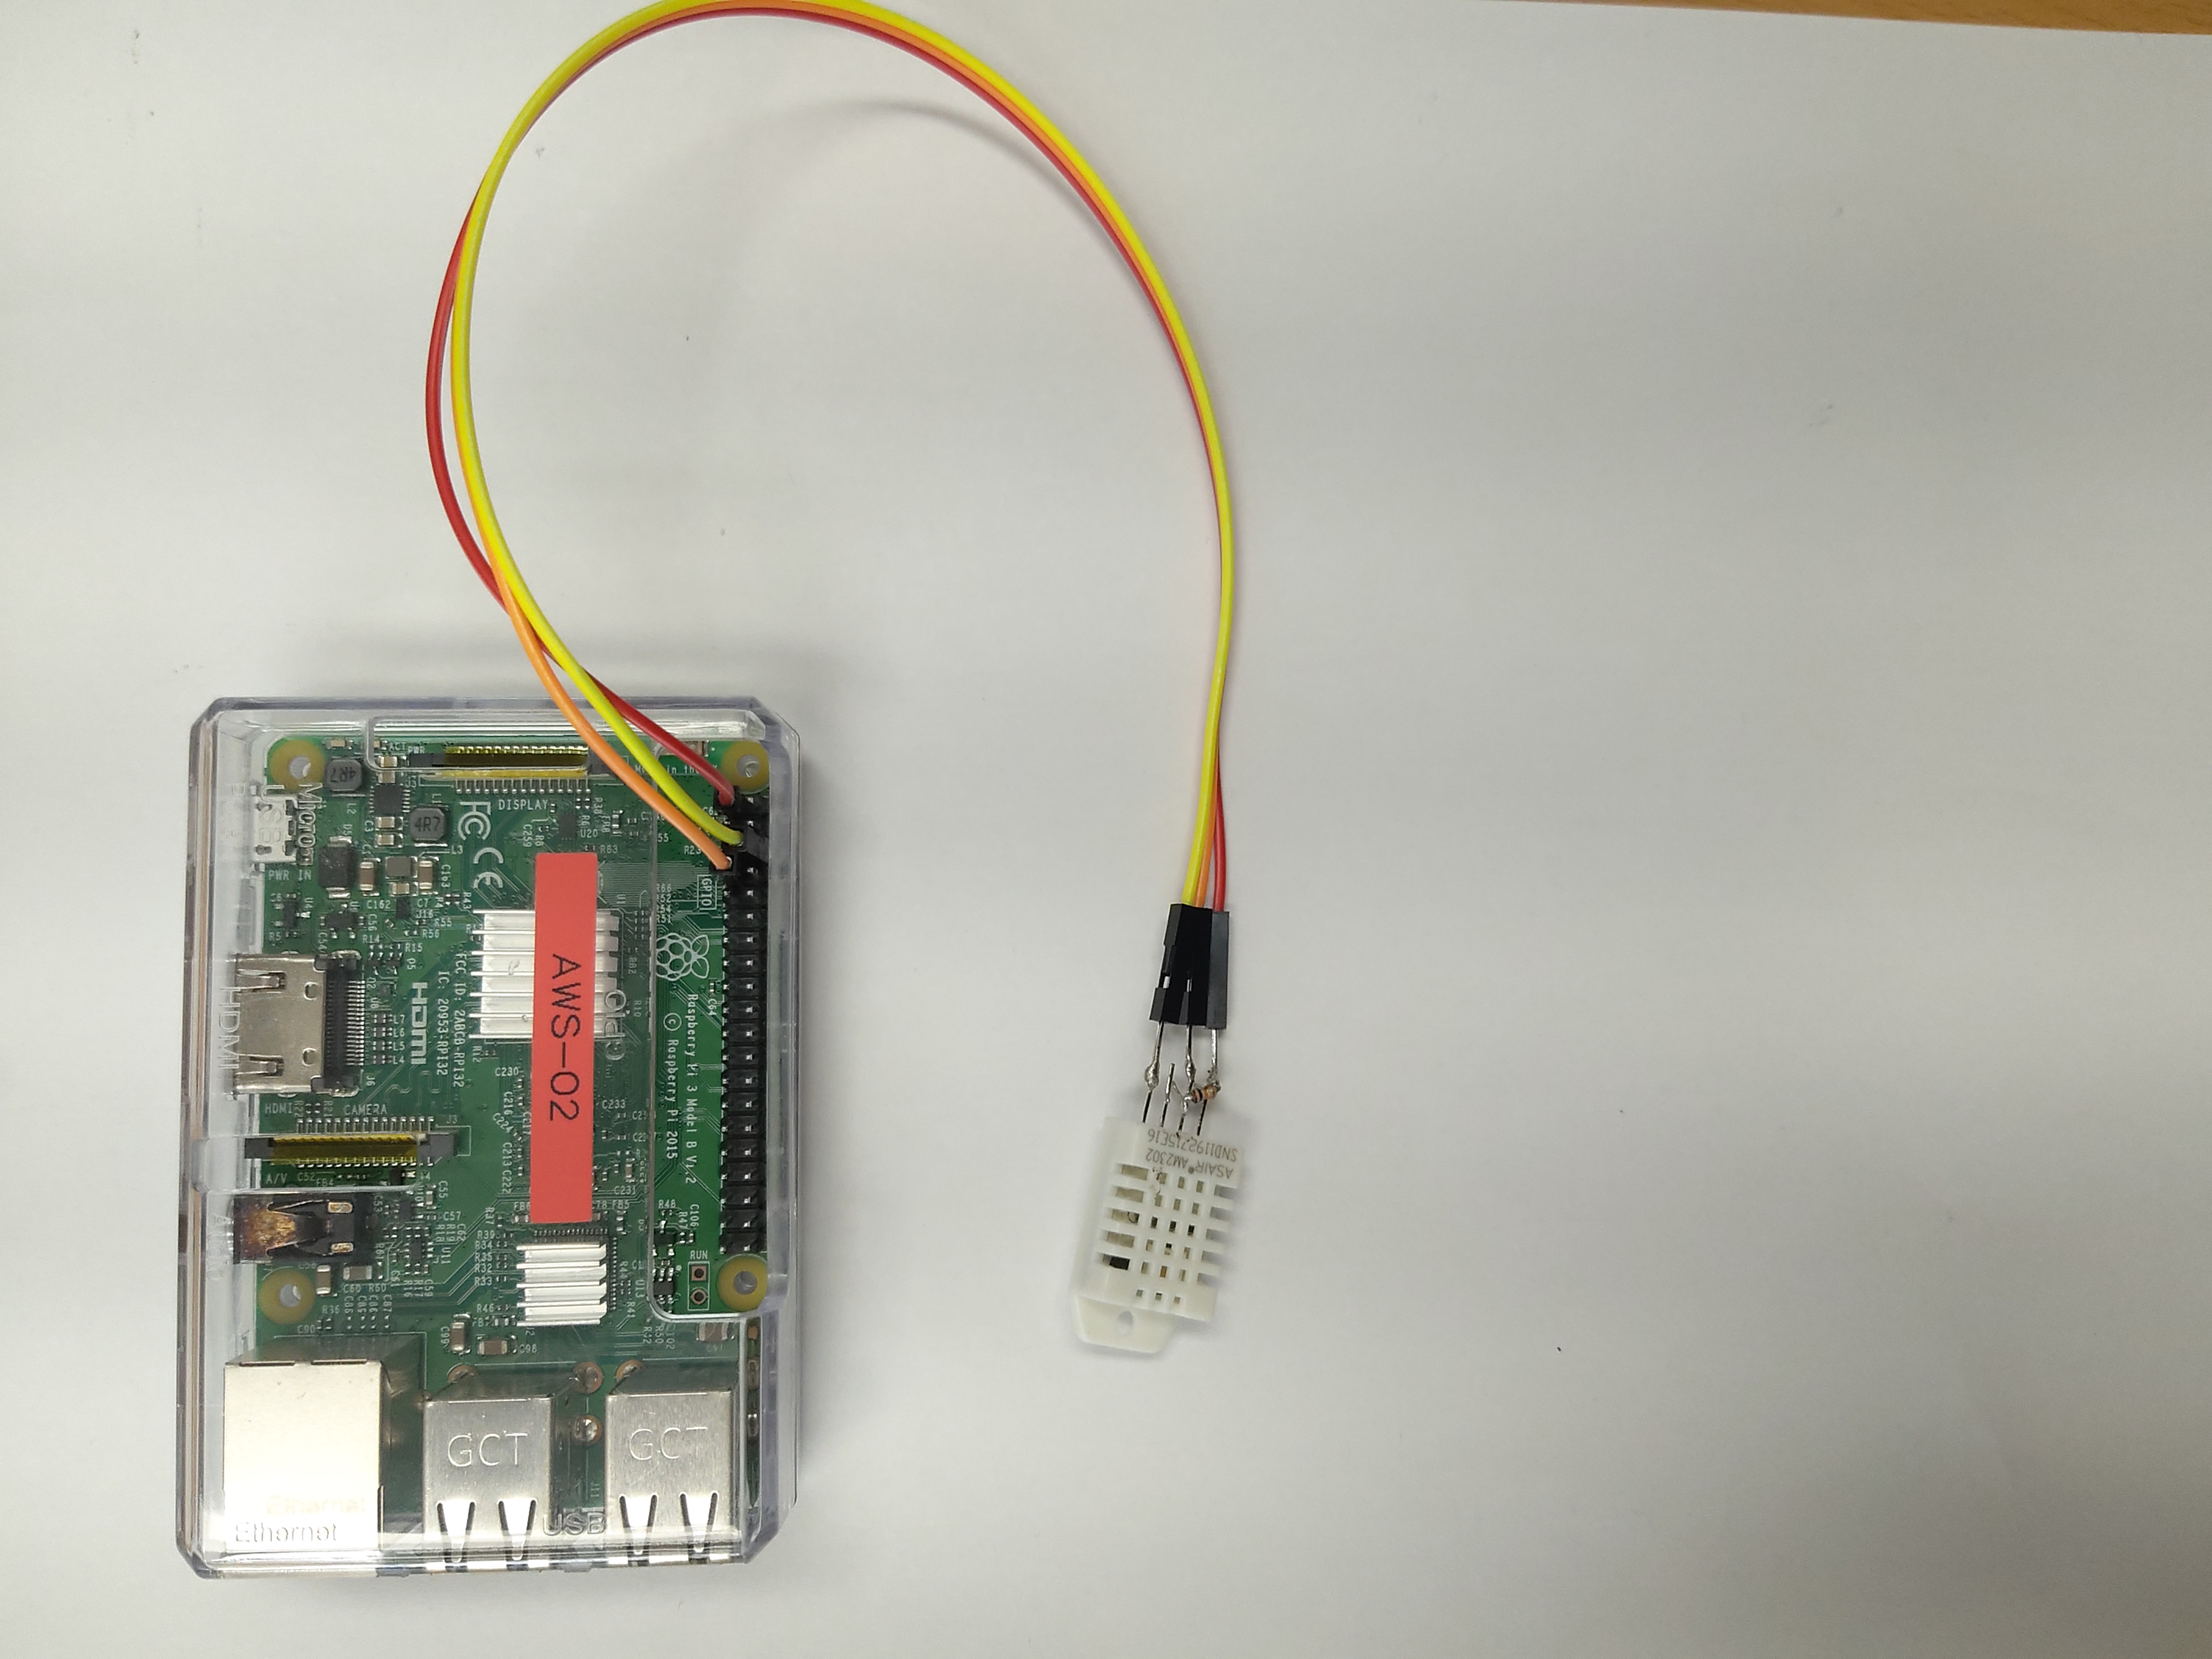
\includegraphics[width=.6\textwidth]{dht22_connect.jpg}
	\caption{DHT22 센서를 단독으로 연결한 모습}
	\label{DHT22}
\end{figure}

\subsubsection{기압 센서(BMP180)}
BMP180은 센서가 위치한 지역의 기압값을 측정하는 센서이며, 온도도 측정 가능하지만 본 연구에서는 이미 온습도 센서가 존재하기에 온도를 측정하는 기능은 사용하지 않았다. BMP180은 3.3 $\textrm{V}$의 입력 전압을 요구하며 2가지 방법으로 통신이 가능하다. BMP180의 통신에는 SPI(Serial Peripheral Interface Bus) 통신을 사용하는 방법과 I2C(Inter-Integrated Circuit) 통신을 사용하는 방법이 존재하였으며 두 방법 모두를 사용하여 연결을 시도해 보았다.
\subsubsection*{SPI 통신 사용}
아래 배선도와 같이 선을 연결하여 사용해 보았다. 3.3 $\textrm{V}$ 핀 1개, 디지털 출력 핀 4개, GND 핀 1개를 요구하며 Python 코드의 실행을 위해 라이브러리를 라즈베리파이에 설치하였다. 코드는 센서에서 받아들인 값을 기압($\textrm{hPa}$ 단위)와 해발고도($\textrm{m}$ 단위)로 환산하여 출력하며 온도는 섭씨온도 단위로 출력한다.

\begin{figure}[htbp]
	\centering
	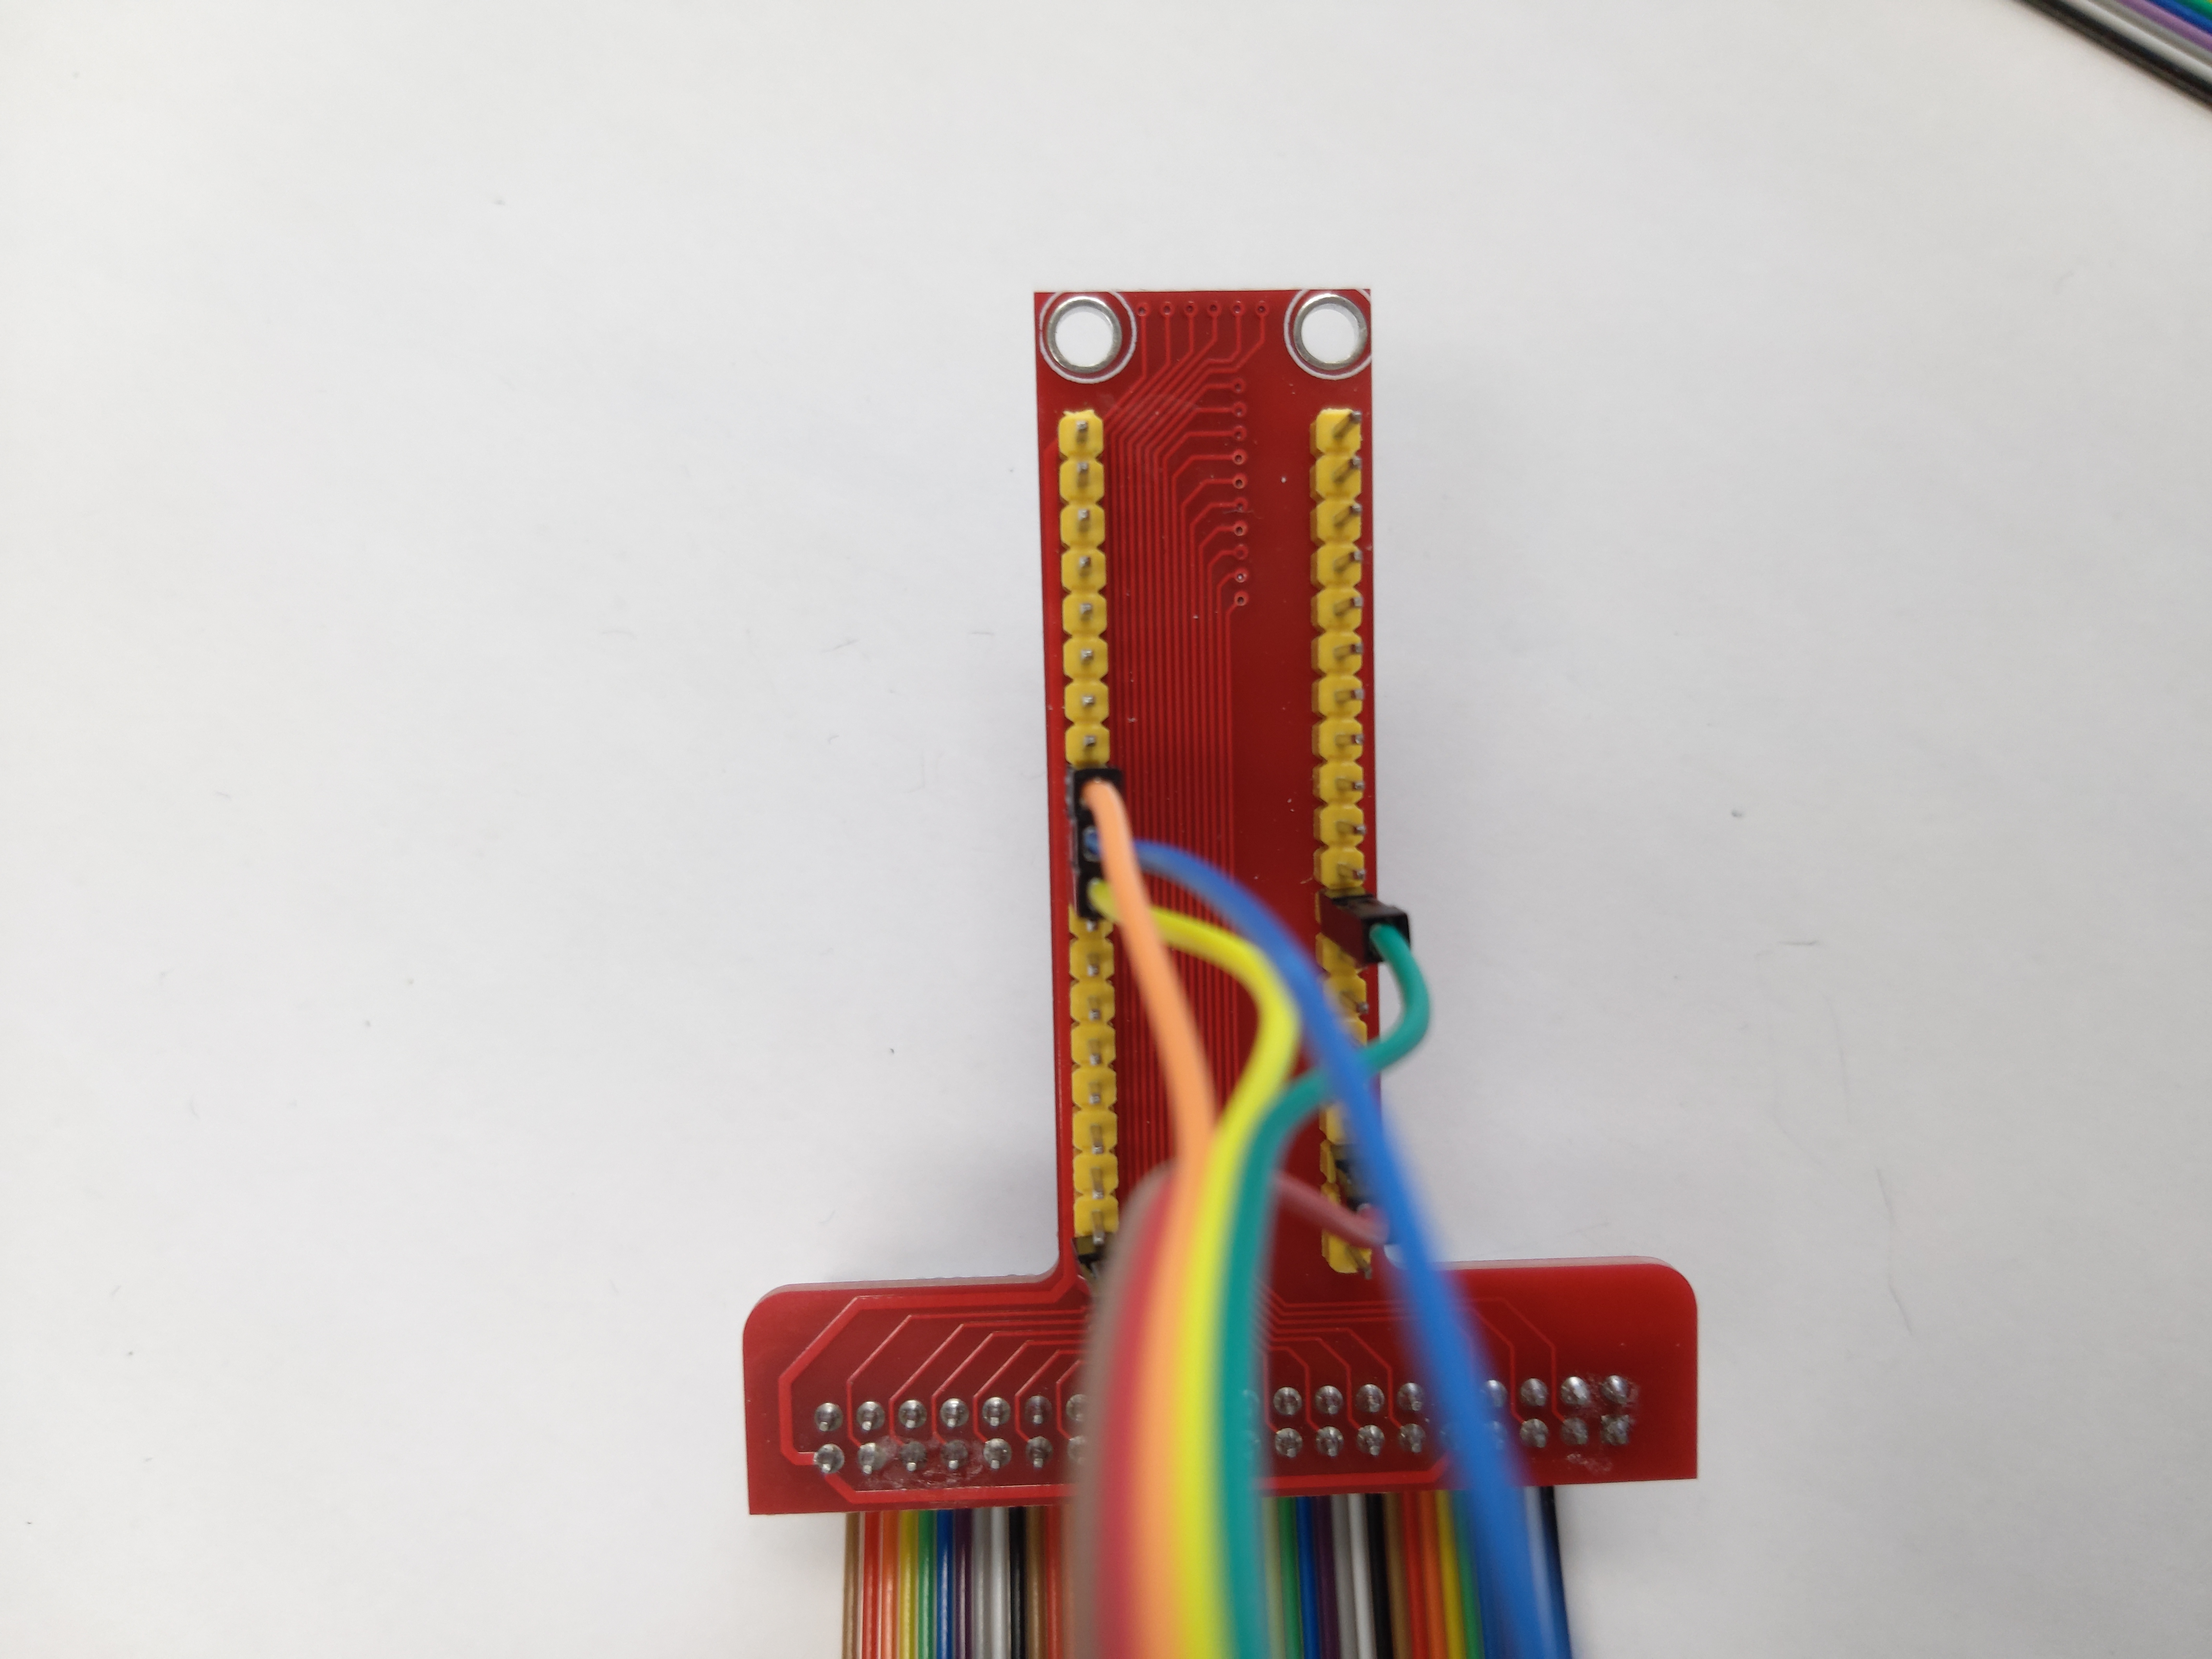
\includegraphics[width=.45\textwidth]{spitest_1}
	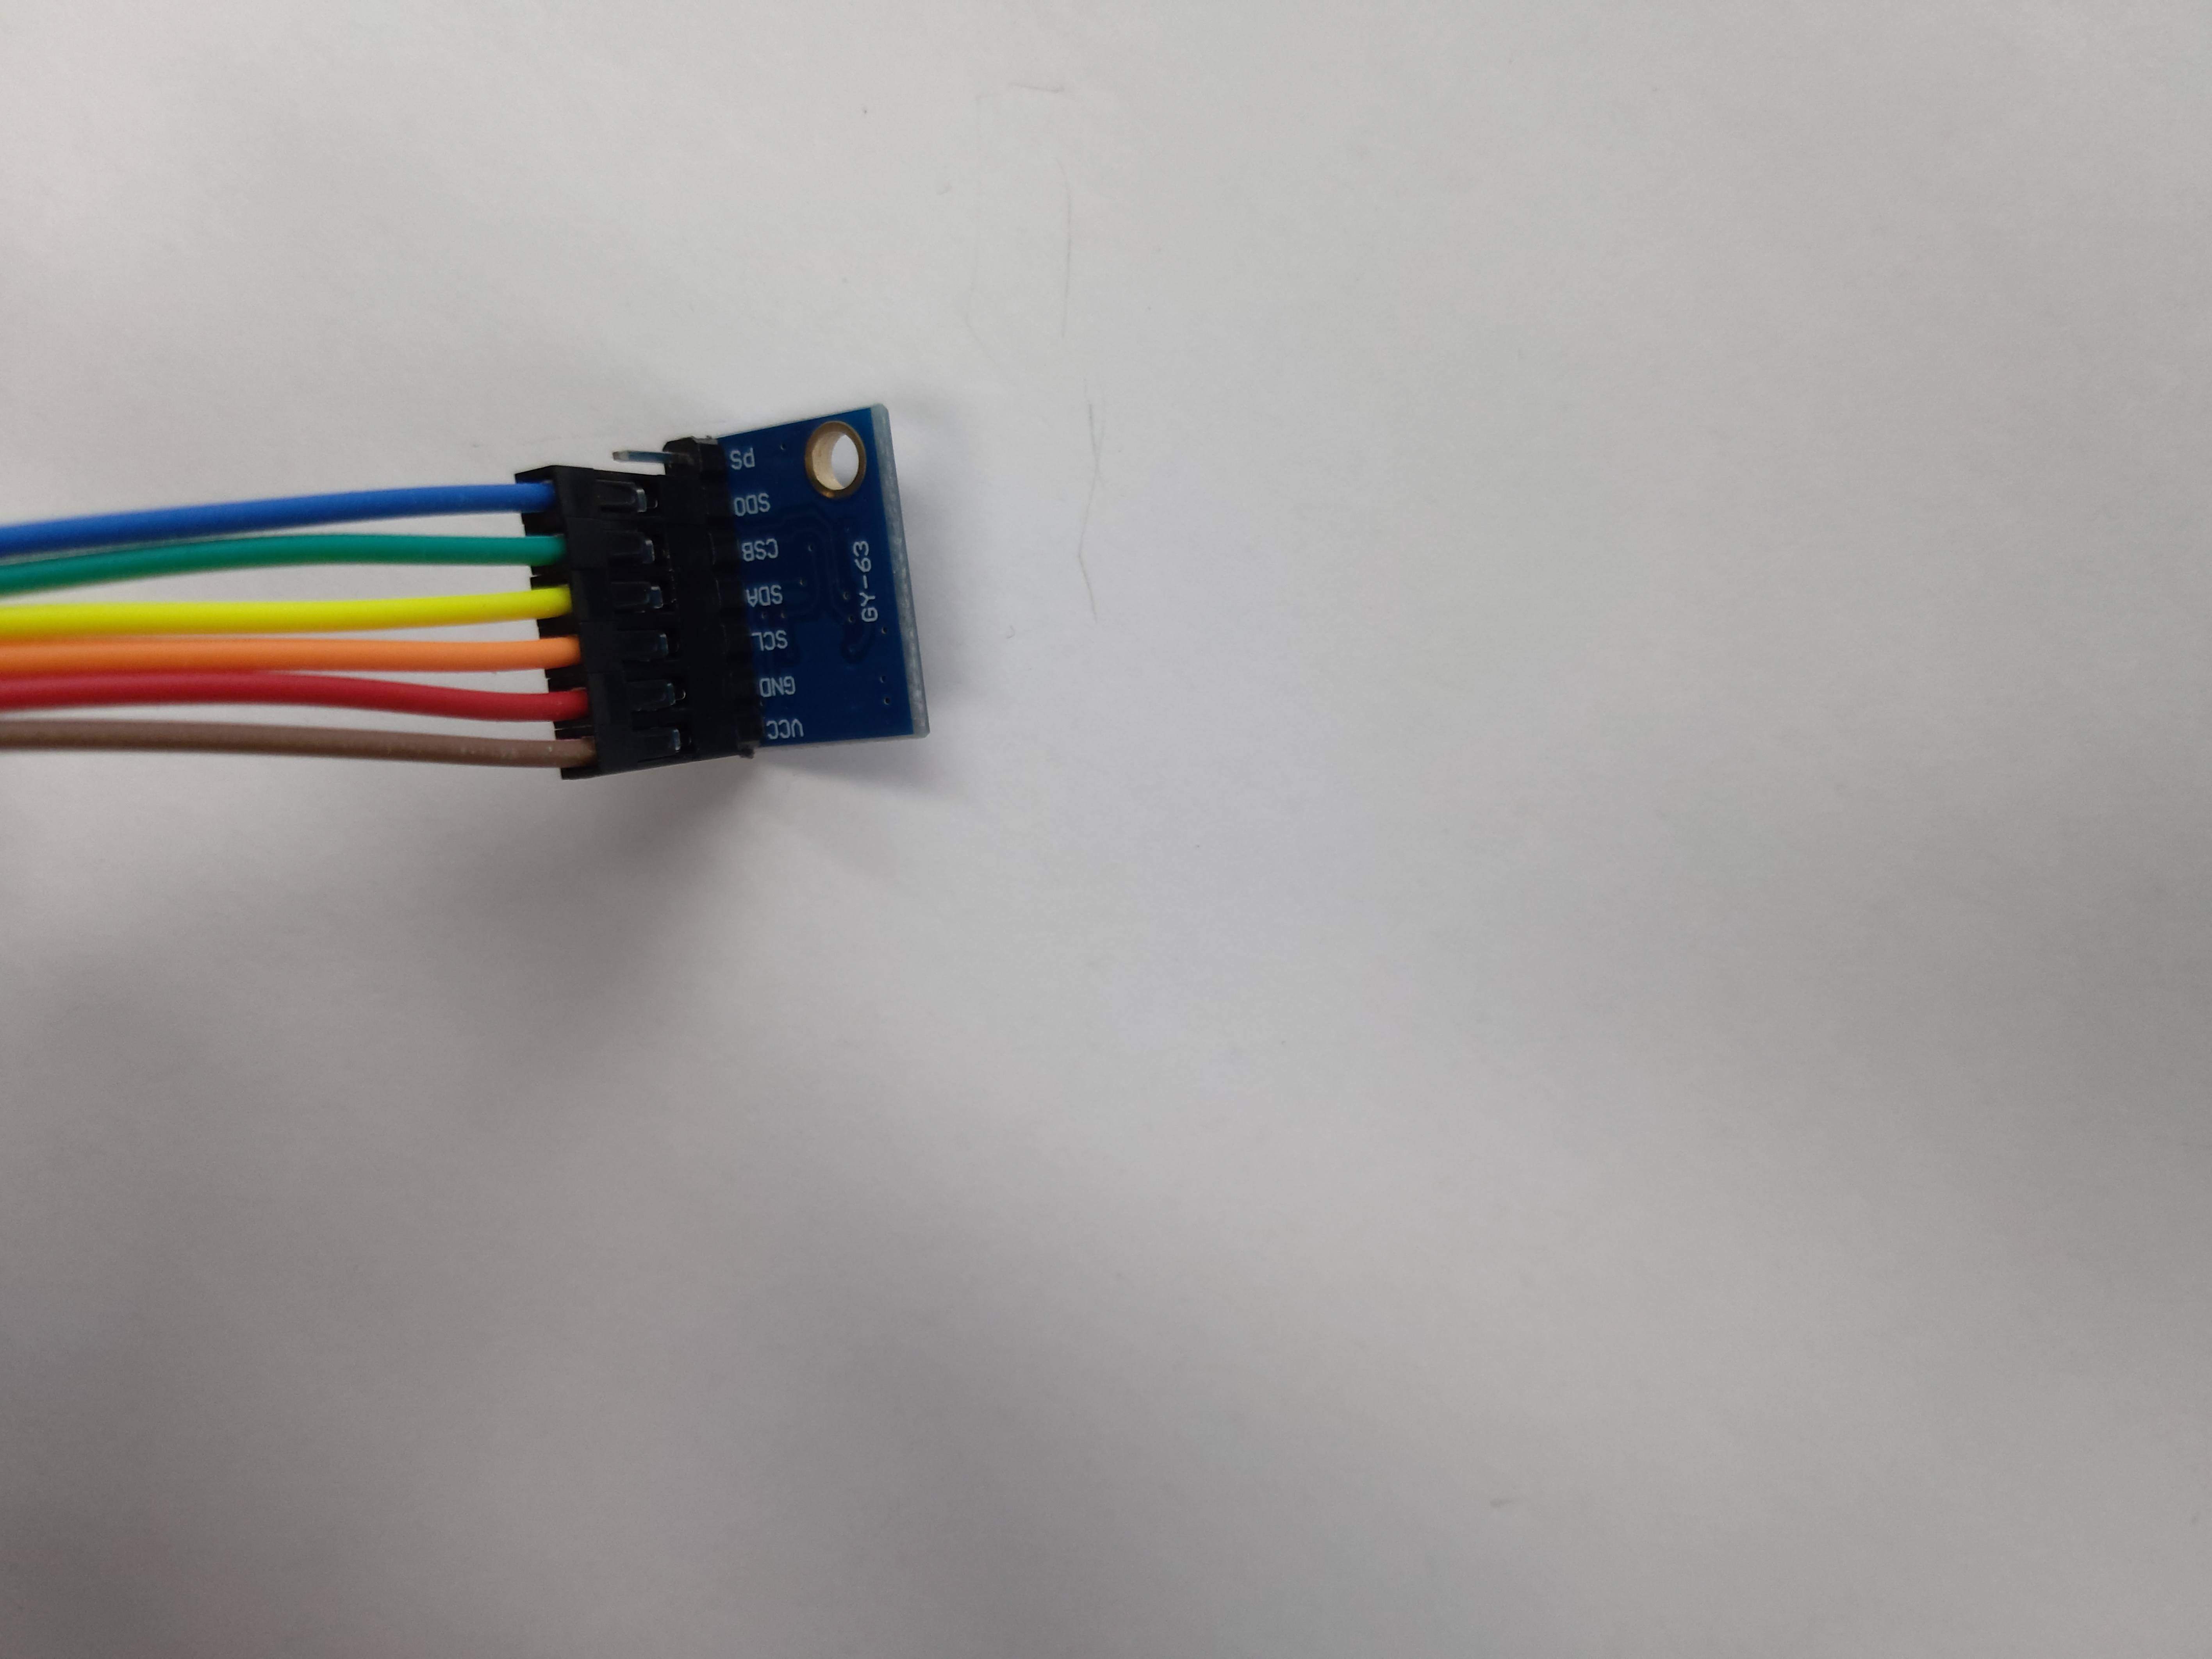
\includegraphics[width=.45\textwidth]{spitest_2}
	\caption{SPI 통신을 사용한 BMP180 센서의 연결}
	\label{SPI}
\end{figure}

\subsubsection*{I2C 통신 사용}
아래 배선도와 같이 전선을 연결하였다. 3.3 $\textrm{V}$ 핀 1개, GND 핀 1개와 디지털 출력 핀 2개를 사용하였으다. 나머지 핀은 연결하지 않는다. Python 라이브러리를 설치 후 코드를 구동해 센서에서 받아들인 값을 기압($\textrm{mba}$ 단위)와 온도(섭씨온도 단위)로 출력하였다.

\begin{figure}[htbp]
	\centering
	\includegraphics[width=.6\textwidth]{pressure}
	\caption{I2C 통신을 사용한 BMP180 센서의 연결}
	\label{I2C}
\end{figure}

\subsubsection{미세먼지 센서(PMS7003)}
미세먼지 센서는 공기 중의 미세먼지 농도를 측정하는 센서이다. 미세먼지는 공기 중에 떠다니는 부피 10㎛³ 이하의 작은 먼지 입자를 일컬어 부르는 말이며 크기가 작아 인체에 흡수된 후 쉽게 제거되지 않아 각종 호흡기 질환을 일으키는 원인이기도 하다. 본 미세먼지 센서는 공기 중의 미세먼지에 의해 빛이 산란되는 원리를 이용해 미세먼지의 대기 중 농도를 측정한다. 이때 측정되는 값은 단위 부피당 질량이 아닌 입자수이므로 미세먼지의 평균 질량에 입자수를 곱해 단위부피당 미세먼지의 질량을 구한다. 

미세먼지 센서는 UART(Universal asynchronous receiver/transmitter) 통신 방식을 사용하기 때문에 GPIO 핀을 사용하여 연결하지 않으며, USB to TTL을 사용해 센서에 전선을 연결하고 그 전선을 케이블을 통해 라즈베리파이의 USB 포트에 연결하여 통신을 한다. 라즈베리파이 3에서 UART 통신은 기본적으로 비활성화되어 있기 때문에 이를 사용하기 위해서는 환경설정에서 활성화시켜줘야 하며, 이를 위해서는 블루투스 통신을 비활성화시켜야 한다.

미세먼지 센서에 인터페이스 보드를 결합한 후, 아래 그림과 같이 4개의 전선을 연결했다. 이 전선을 USB to TTL 케이블에 연결한 후, 케이블을 라즈베리파이에 연결했다. 그 후 미세먼지서버가 연결된 UART를 확인하고 Python 코드에서 UART명을 입력하는 부분에 현재 센서가 연결된 UART를 입력했다. 결과값 표출 명령어는 PMS7003의 데이터시트와 제공되는 예시 코드를 변형하여 사용하였다.

\begin{figure}[htbp]
	\centering
	\includegraphics[width=.6\textwidth]{pms7003_connect.jpg}
	\caption{PMS7003 센서를 USB to TTL 케이블을 사용해 연결한 모습}
	\label{PMS7003}
\end{figure}

\subsubsection{ADC(Analog to Digital Converter, MCP3208)}
풍향센서와 풍속센서는 각각 바람의 세기와 방향에 따라 결과를 연속적인 전압 값으로 출력하며 이 값을 읽어들이기 위해서는 아날로그 통신이 필요하다. 그러나 라즈베리파이의 GPIO 핀 중에는 아날로그 통신이 가능한 핀이 없기 때문에 아날로그 신호를 디지털로 바꿔주는 ADC, 즉 아날로그-디지털 변환기를 사용해 값을 받아들인다. 

본 연구에서 사용하는 ADC인 MCP3208은 아날로그 입력값을 받아들이는 8개의 핀과 그 값을 라즈베리파이에 전송하기 위해 사용하는 8개의 핀으로 구성되어 있다. ADC를 라즈베리파이에 다음 그림과 같이 연결했으며 C언어와 Python을 각각 사용해 구동시켜 보았다.

\begin{figure}[htbp]
	\centering
	\includegraphics[width=.6\textwidth]{adc_connect}
	\caption{ADC(MCP3208)을 라즈베리파이에 연결한 모습}
	\label{ADCCON}
\end{figure}

\subsubsection{풍속센서(SEN0170)}
풍속센서는 바람이 흐르는 속력을 측정하는 센서이다. 풍속센서의 풍속계는 바람이 세게 불수록 더 빨리 회전하며, 이 회전하는 정도를 연속적인 전압값으로 출력한다. SEN0170의 데이터시트에는 풍속이 0 $\textrm{m/s}$일 때 출력 전압이 0.4 $\textrm{V}$, 풍속이 32.4 $\textrm{m/s}$ 때의 출력 전압이 2.0 $\textrm{V}$로 표시되어 있었다. 32.4 $\textrm{m/s}$는 본 센서가 측정할 수 있는 최대 풍속이며 그러므로 출력되는 최대 전압은 2.0 $\textrm{V}$를 넘지 않는다. 

본 연구에서는 전압과 풍속의 상관관계가 선형적이라고 가정한 뒤 전압에 따른 풍속을 구하는 공식을 도출하였다. 전압을 $V$ [V], 풍속을 $v$ [m/s]라 할 때 둘 사이에는
\[ v=20.25V-8.1\quad (V\geq 0.4\textrm{V})\]
의 관계가 성립함을 알 수 있었다. 이때 전압이 0.4 $\textrm{V}$ 미만이라면 풍속은 0 $\textrm{m/s}$로 표시하도록 하였다.
풍속센서에는 4개의 전선이 존재한다. 2개는 각각 (+)와 GND를 연결하는 전선이며, 1개는 전압을 출력하는 전선이고, 나머지 1개의 전선은 사용하지 않는다. 

데이터시트에 의하면 풍속센서는 7$\sim$24 $\textrm{V}$의 직류 전압 사이에서 동작하므로 12 $\textrm{V}$ 배터리에 센서를 연결하여 사용하기로 하였다. (+)극 선과 GND 선을 12 $\textrm{V}$ 배터리에 연결할 수 있도록 케이블과 납땜하였으며, 풍속센서의 출력 전선을 ADC의 CH0(아날로그 전압값을 읽어들이는 핀)에 연결한 후 명령어를 작성하고 실행해 풍속이 올바르게 표출되는지 확인하였다. 명령어는 ADC에서 사용한 코드에서 읽어들인 전압값을 이용해 풍속을 계산하여 출력하도록 하였다.

\subsubsection{풍향센서(DM2014)}
풍향센서는 바람이 부는 방향을 출력하는 센서이다. 데이터시트에 의거하면 풍향센서는 바람이 부는 방향에 따라 16방위로 나누어 각 방위에 따라 전압값을 다르게 표현하며, 이를 이용해 바람이 불어오는 방향을 알 수 있다. 

풍향센서에는 4개의 핀이 존재하며 2개는 각각 (+)극과 GND를 연결하는 선이고 1개는 전압을 출력하는 전선, 나머지 1개는 사용하지 않는 전선이다. 풍향센서의 동작전압은 12$\sim$24 $\textrm{V}$ 사이의 직류 전압이므로 (+)극 선과 GND 선이 배터리에 연결될 수 있도록 전선을 케이블에 납땜한 뒤 12 $\textrm{V}$의 배터리에 풍향센서를 연결하였다. 명령어를 작성하고 구동하기 전에 멀티미터를 사용하여 바람의 방향이 변함에 따라 전압값이 제대로 출력하는지 확인하였다. 멀티미터를 사용하여 GND 핀과 출력 전압 핀 사이의 전압을 측정하였다.

\begin{figure}[htbp]
	\centering
	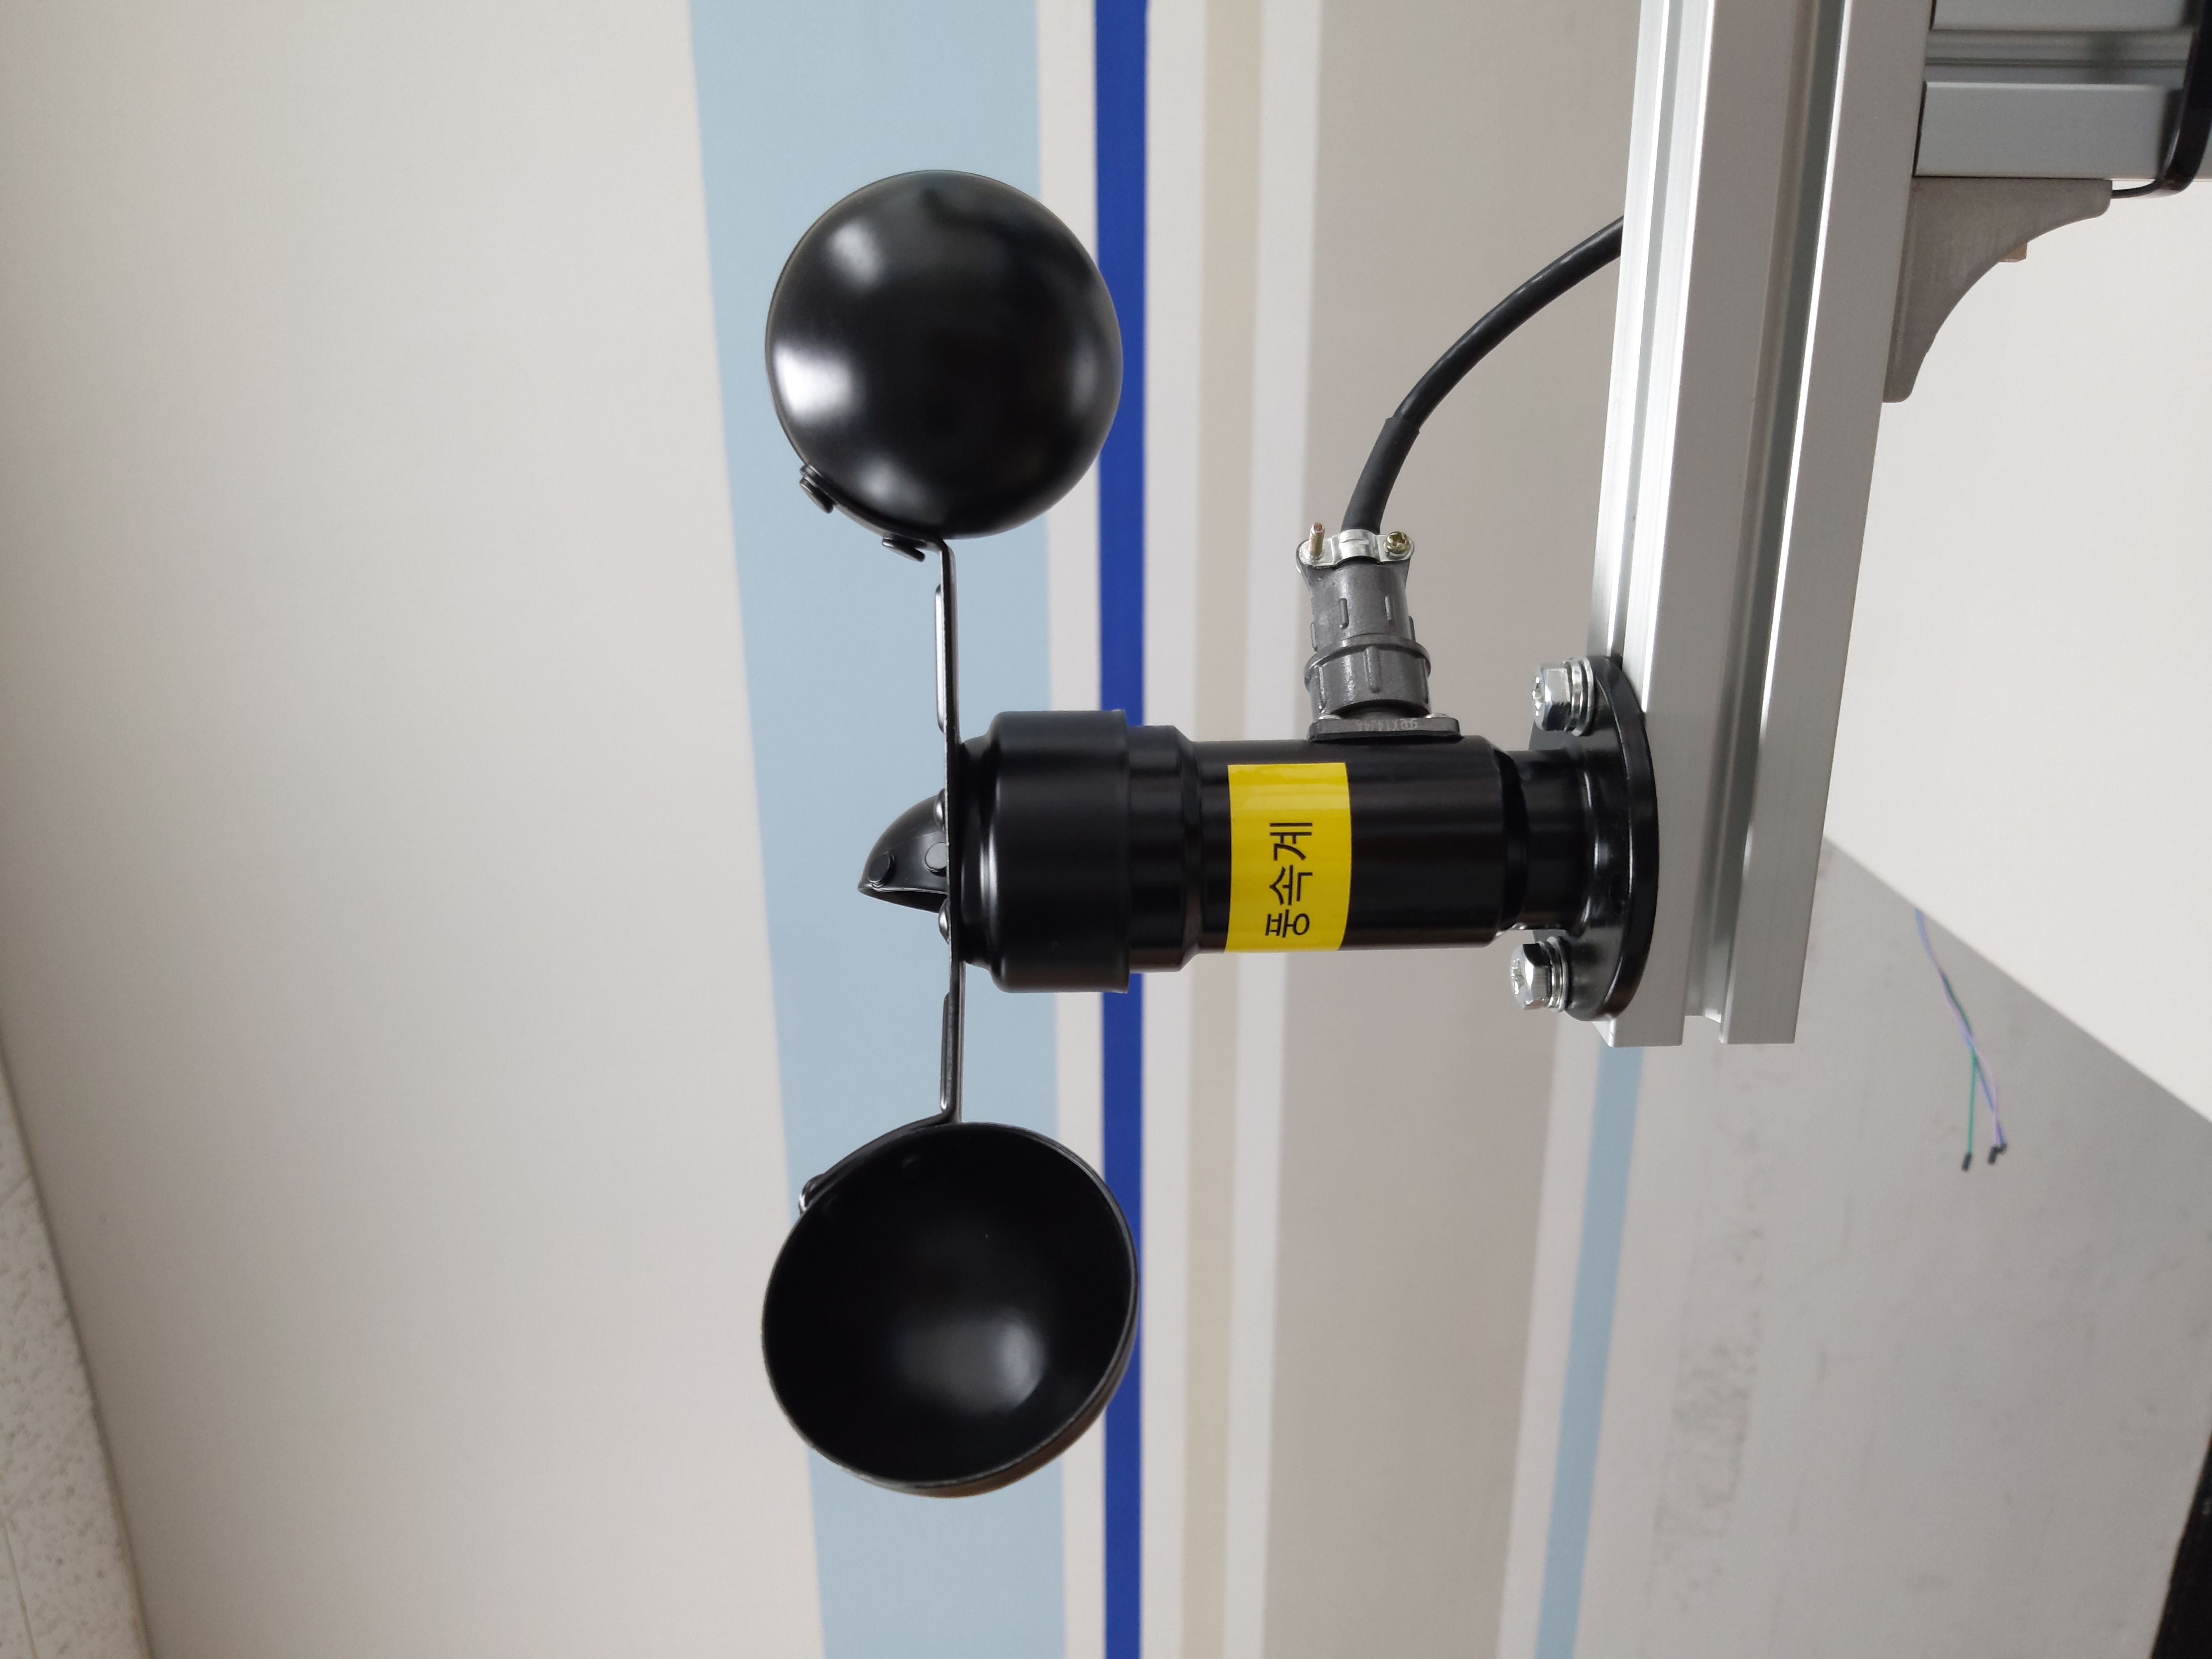
\includegraphics[width=.45\textwidth]{windspeed}
	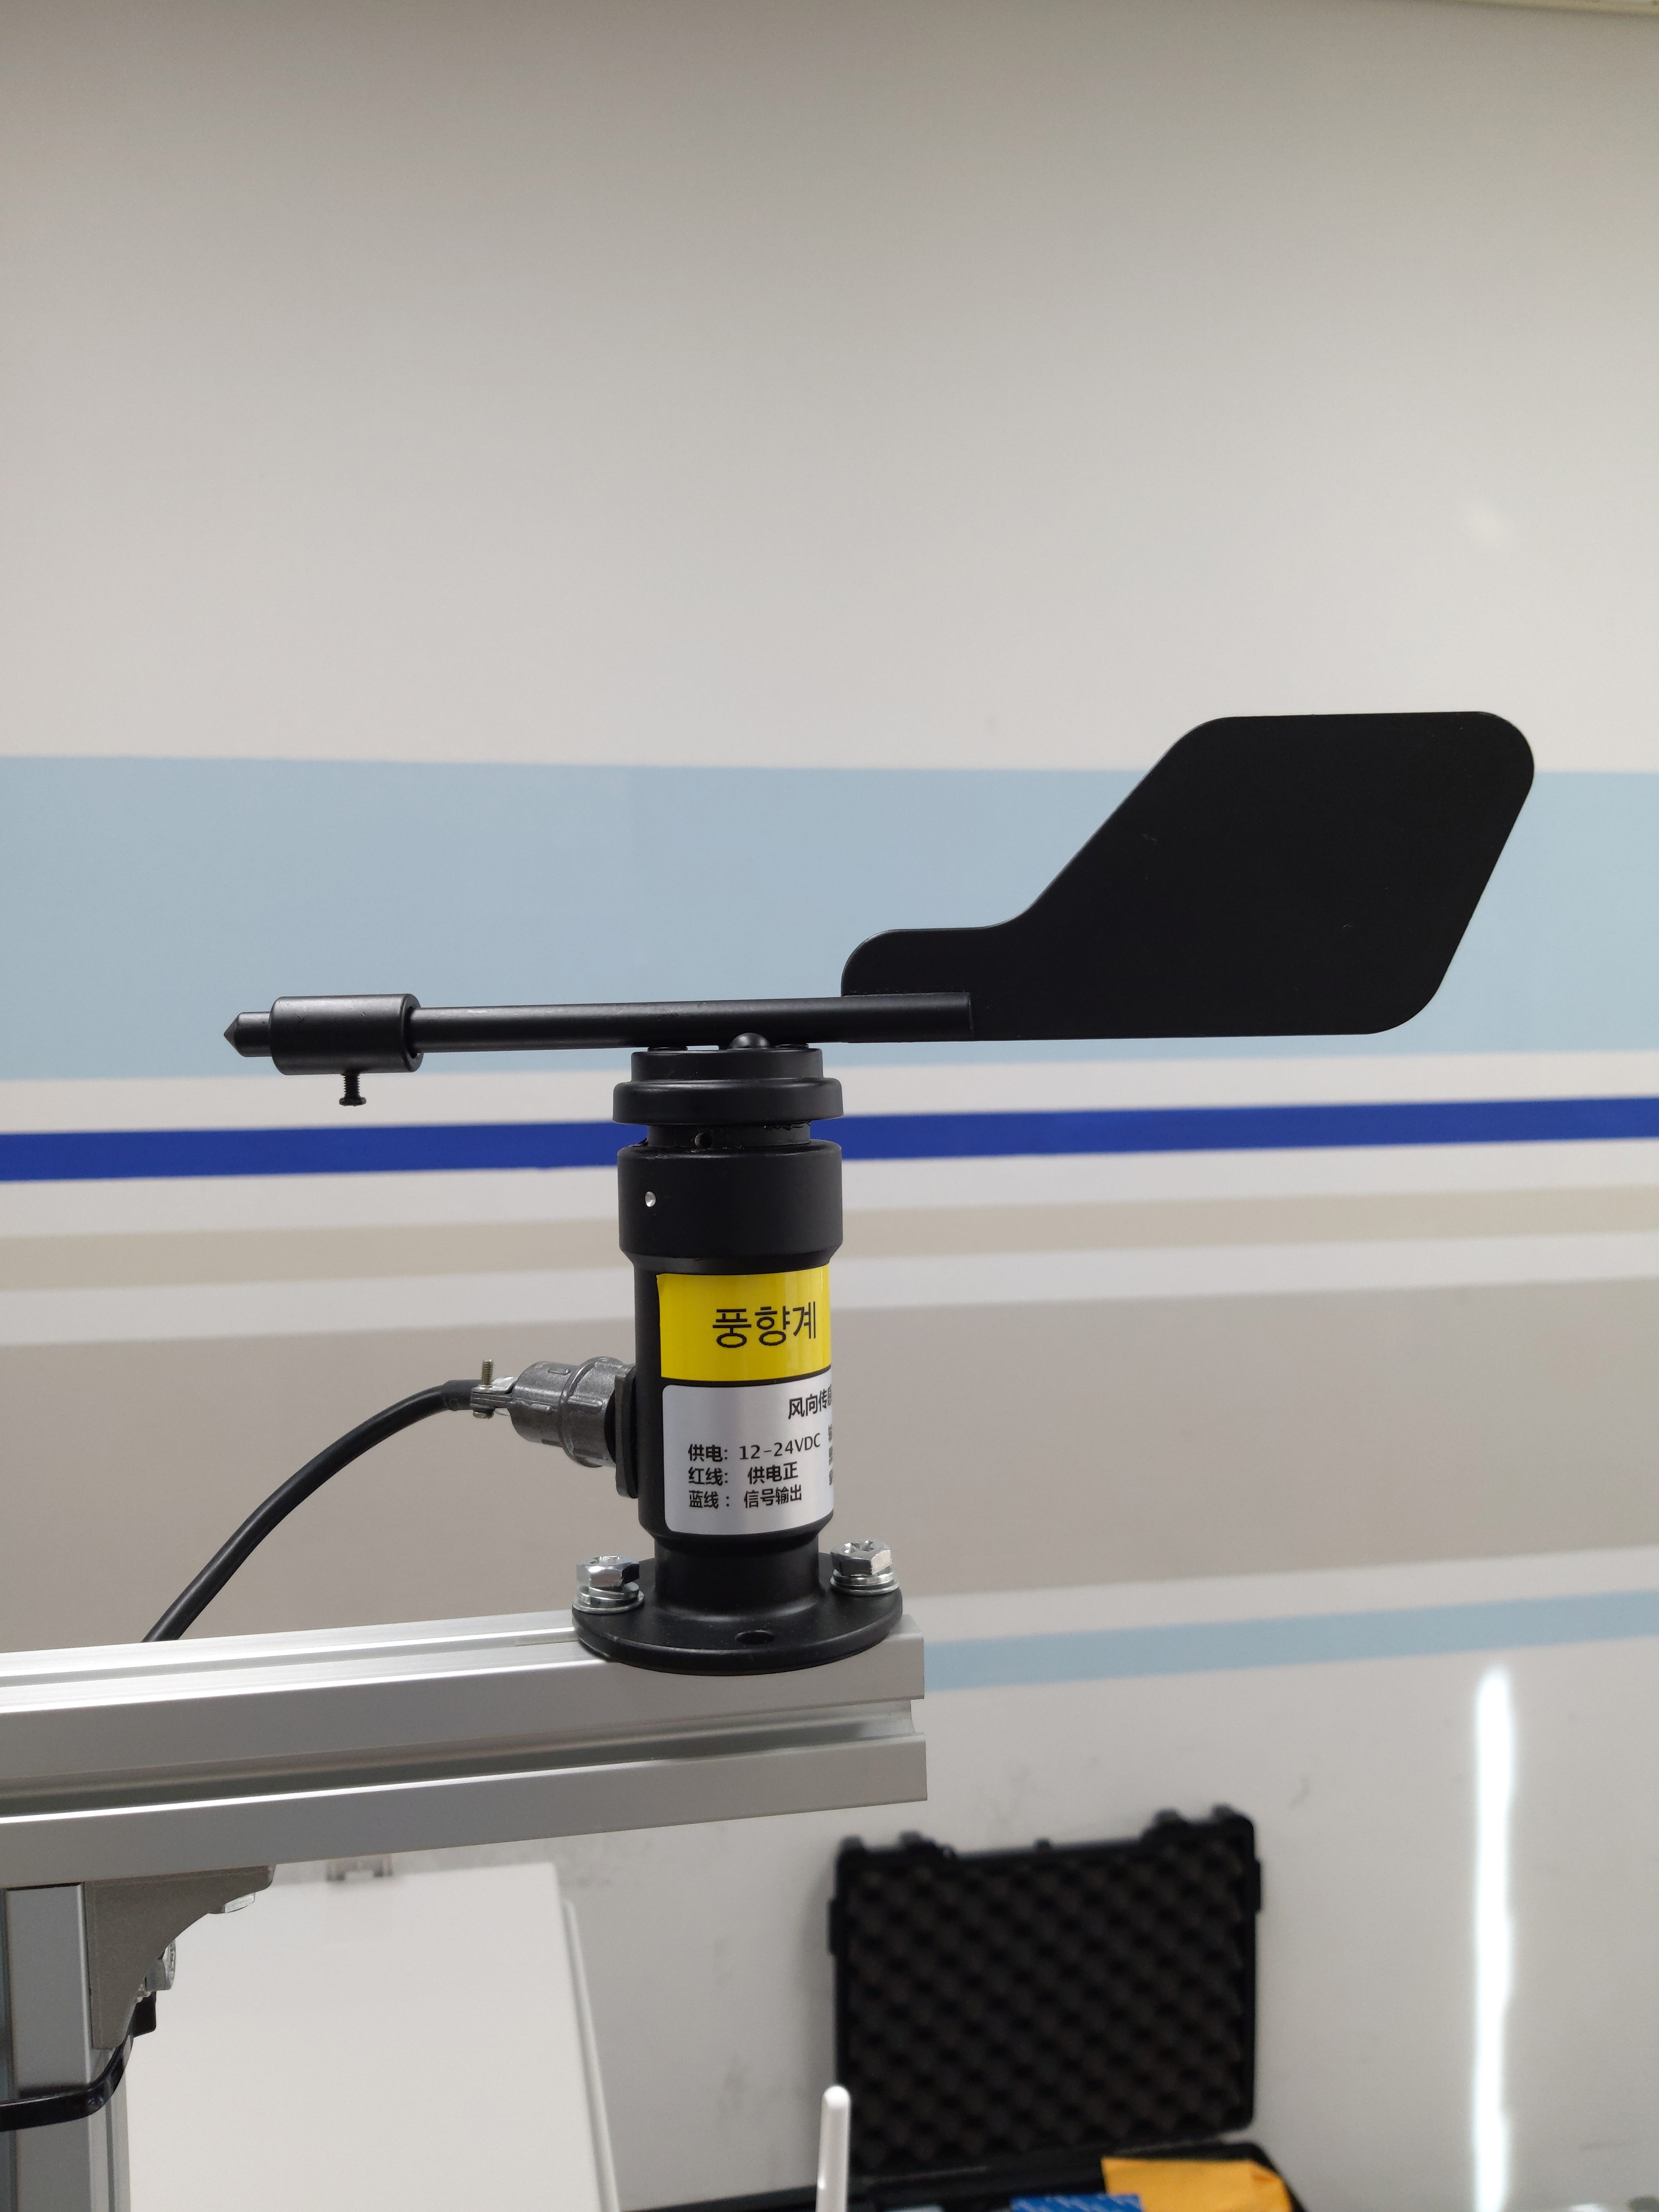
\includegraphics[width=.45\textwidth]{winddir}
	\caption{풍속센서와 풍향센서의 모습}
	\label{WIND}
\end{figure}

\subsubsection{강우량센서(p/n 80422)}
강우량센서는 빗방울이 떨어질 때만 전기 신호가 전달되는 방식으로 강우량을 측정하는 센서이다. 강우량센서에 빗방울이 떨어지면 강우량센서의 하부에 위치한 시소 모양의 건축물이 기울어지게 된다. 이에 따라 버튼이 눌려지고, 버튼이 한 번 눌려질 때마다 신호가 전달되어서 버튼이 눌린 횟수에 따라 내린 비의 양을 알 수 있게 된다. 

센서는 강우량을 비 한 방울의 부피와 버튼이 눌러진 횟수를 곱해 구한다. 강우량 센서의 전선을 다음과 같이 연결한 후 명령어를 작성해 실행 여부를 확인했다. 강우량 센서에 빗방울이 떨어진 경우에만 프로그램이 값을 출력하게 되어 있어 비가 내리지 않는 경우 아무런 값도 출력하지 않는다.

\begin{figure}[htbp]
	\centering
	\includegraphics[width=.6\textwidth]{rainfall}
	\caption{강우량센서를 라즈베리파이에 연결한 모습}
	\label{RAINFALL}
\end{figure}

\subsection{AWS 구조물의 보수와 센서의 기판 연결}
본교의 SRC(Science Research Center) 7층 야외에 위치해 있으나 현재 사용하지 않는 AWS 구조물을 보수하고 센서와 전선을 연결했다. 과거 AWS 구조물은 알루미늄 프로파일을 이용해 제작되였으며 양쪽 벽면에 와이어를 이용해 고정시킨 상태였으나 붕괴된 적이 있어 추가적인 보수가 필요한 상황이었다. 본 연구에서는 알루미늄 프로파일의 접합부에 볼트와 너트를 2중으로 설치하였으며, 구조물의 양쪽을 와이어를 사용해 다시 벽에 단단하게 고정하였다. 또한 구조물의 상단부에 풍속 센서와 풍향 센서를 설치하고 전선을 케이블 타이로 알루미늄 프로파일에 고정하였다. 구조물의 측면에는 태양광 전지판을 설치했다. 

구조물의 중간 부분에는 라즈베리 파이와 배터리, 풍향, 풍속, 강수량을 제외한 각종 센서가 위치할 공간이 위치해 있다. 상자에 라즈베리 파이와 온습도, ADC, 기압 센서를 연결한 기판을 놓은 후 상자에 펀치를 이용해 전선이 들어갈 구멍을 뚫었다. 그 후 배터리와 상자를 구조물 위에 놓고 풍속, 풍향, 강우량 센서의 전선과 배터리의 전선을 상자 안에 넣어 라즈베리파이와 연결했다.

풍향과 미세먼지 센서를 제외한 모든 센서의 전선과 ADC, 라즈베리파이 확장 보드(GPIO Extension Board)를 만능기판에서 서로 납땜하여 연결했다. 라즈베리파이 확장 보드는 라즈베리파이에 연결하였을 경우 라즈베리파이에 기본적으로 내장되어 있는 핀과 동일한 용도로 사용할 수 있으며 전선의 연결과 납땜, 이후 유지 보수를 쉽게 해주는 역할을 한다.

\subsection{서버 데이터베이스로 수집한 정보 전송}
김용남, 성기훈, 홍정희, 강동일 (2009)은 자동기상관측장비에서 수집한 데이터를 표출하는 웹 페이지를 개발하는 연구를 진행하였으나 이는 미리 설치되어 있던 AWS에서 값을 받아와 웹 페이지에 표출하는 형태였다\cite{Ref2}. 

본 연구에서는 MariaDB를 통해 라즈베리파이를 이용하여 직접 수집한 기상 정보를 체계적으로 정리할 데이터베이스를 구축한 후 이를 웹상에서 관리하기 위해 경기과학고 지구과학 홈페이지에 설치된 phpMyAdmin(ess.gs.hs.kr/phpmyadmin)을 이용하였다. 서버에 기상 정보를 저장하는 DB인 AWS\_GSHS를 만든 후 아래와 같이 테이블을 제작하였다. 테이블의 이름은 1min\_data로 하였으며 내용은 기상청 날씨누리에서 제공하는 AWS 관측자료의 형식을 따랐다. 단 본 연구에서 제작한 AWS 장비에서 현재 측정할 수 없는 자료는 NULL값을 기본으로 저장하기로 설정하였다.

라즈베리파이에서 수집한 값을 서버에 전송하기 위해 Python에서 pymysql 모듈을 불러온 후 SQL문을 사용하였다. C언어와 Python 명령어에서 반복문을 실행하는 시간 간격이 같도록 프로그램의 시간 딜레이를 설정하였다. 또한 수집한 정보는 라즈베리파이 내부에도 csv(comma separated value) 파일의 형태로 저장하도록 설정하였다.

% Please add the following required packages to your document preamble:
% \usepackage{graphicx}
\begin{table}[htbp]
	\caption{AWS\_GSHS DB의 1min\_data 테이블 구조}
	\label{DBTable}
	\resizebox{\textwidth}{!}{%
		\begin{tabular}{c|c|c|c|c}
			\toprule
			이름            & 설명            & 데이터형    & 기본값  & 비고            \\ 
			\toprule
			id            & 데이터 일련번호      & int     &      & 자동으로 부여       \\ \hline
			OBS\_code     & AWS 지역코드      & int     &      & 임의로 111111 부여 \\ \hline
			OBS\_datetime & 측정시각          & varchar &      & 연월일-시분초로 표시   \\ \hline
			preci\_now    & 현재 강수여부       & varchar &      & O, X로 표시      \\ \hline
			preci\_15     & 15분 누적강우량     & float   &      &               \\ \hline
			preci\_60     & 60분 누적강우량     & float   &      &               \\ \hline
			preci\_3H     & 3시간 누적강우량     & float   &      &               \\ \hline
			preci\_6H     & 6시간 누적강우량     & float   &      &               \\ \hline
			preci\_12H    & 12시간 누적강우량    & float   &      &               \\ \hline
			preci\_1day   & 1일 누적강우량      & float   &      &               \\ \hline
			temperature   & 기온            & float   &      &               \\ \hline
			wind\_dir011  & 1시간 풍향(360도)  & float   & NULL &               \\ \hline
			wind\_dir012  & 1시간 풍향(16방위)  & float   & NULL &               \\ \hline
			wind\_spd01   & 1시간 풍속        & float   &      &               \\ \hline
			wind\_dir101  & 10시간 풍향(360도) & float   & NULL &               \\ \hline
			wind\_dir102  & 10시간 풍향(16방위) & float   & NULL &               \\ \hline
			wind\_spd10   & 10시간 풍속       & float   & NULL &               \\ \hline
			RH            & 상대습도          & float   &      &               \\ \hline
			Air\_P        & 대기압           & float   &      &               \\ \hline
			REMARK        & 비고            & varchar &      & ‘RnE’로 표시     \\ 
			\toprule
		\end{tabular}%
	}
\end{table}